% Camera-ready version for PanAfriCon AI 2026 (Springer CCIS), built on the
% Springer LLNCS template v2.25. Condensed from ../manuscript.tex (the extended
% version); all counts and inclusion rules are identical. Compile with pdfLaTeX,
% as in the template; the Ge'ez word is included as geez_salam.pdf.
\documentclass[runningheads]{llncs}

\usepackage[T1]{fontenc}
% T1 fonts will be used to generate the final print and online PDFs (LLNCS template).
\usepackage{newtxtext}
\usepackage[varvw]{newtxmath}

\usepackage{graphicx}
% The Ge'ez word in Sect. 1, pre-rendered as a vector graphic (see geez_salam.tex)
\newcommand{\geezsalam}{\raisebox{-0.1ex}{
\includegraphics[height=1.55ex]{geez_salam.pdf}}}
\usepackage{cite}
\usepackage{booktabs}
\usepackage{tabularx}
\usepackage{array}
\usepackage{tikz}
\usetikzlibrary{positioning,arrows.meta}
\usepackage{hyperref}
\usepackage{xurl}
\usepackage{color}
\renewcommand\UrlFont{\color{blue}\rmfamily}
\urlstyle{rm}
\emergencystretch=1.5em

\begin{document}

\title{Foundational NLP Tools for Ge'ez-Script Languages: A Systematic Tool-Centred Analysis}
\titlerunning{Foundational NLP Tools for Ge'ez-Script Languages}

\author{Hailay Kidu Teklehaymanot\inst{1,2}\thanks{Corresponding author.} \and
Gebreagziher Gebrelibanos Mesfun\inst{3} \and
Tsegaye Semere Gebremichael\inst{4} \and
Gebrearegawi Gebremariam\inst{5} \and
Alemu Kumilachew Tegegnie\inst{6} \and
Nesina Gr\"{u}tter\inst{2}}
\authorrunning{H. K. Teklehaymanot et al.}

\institute{L3S Research Center, Leibniz University Hannover, Hannover, Germany\\
\email{teklehaymanot@l3s.de} \and
University of Zurich, Zurich, Switzerland\\
\email{hailaykidu.teklehaymanot@uzh.ch} \and
Adigrat University, Adigrat, Ethiopia \and
National Tsing Hua University, Hsinchu, Taiwan \and
Axum University, Axum, Ethiopia \and
Bahir Dar University, Bahir Dar, Ethiopia}

\maketitle

\begin{abstract}
The Ge'ez script is used to write several languages of the Horn of Africa. This survey covers three of them: Amharic and Tigrinya, spoken by tens of millions of people in Ethiopia and Eritrea, and Classical Ge'ez, the liturgical language of the Ethiopian and Eritrean Orthodox Tewahedo and Catholic Churches. These languages remain underrepresented in natural language processing (NLP) research. We present a systematic, tool-centred survey organised around four pillars: (i)~tokenisation and normalisation; (ii)~morphological analysis and synthesis; (iii)~text representation, embeddings, and evaluation; and (iv)~sequence labelling and structure extraction. A dual inclusion standard governs the survey: papers enter the literature corpus through a peer-review track or, if they release a checkable artefact, a provenance track, while tools enter the inventory on public provenance alone. Guided by PRISMA 2020, we review 69 verified publications (2017--2026) and report 28 foundational tools, models, datasets, and linguistic resources confirmed publicly available on GitHub, Zenodo, PyPI, or HuggingFace as of 21 September 2026; 26 trace to a corpus paper and two are provenance-track additions. Amharic is the most represented language in both the literature and the inventory, Tigrinya second, and Classical Ge'ez least. Tokenisation and morphology are the least-served pillars, while embeddings and evaluation dominate. Eight tools cover more than one of the three languages, but none is a script-level transfer framework, and they share no annotation or evaluation standard. We close with seven research priorities. Data and verification code: \url{https://github.com/hailaykidu/geez-nlp-survey}.

\keywords{Ge'ez script \and Low-resource NLP \and Amharic \and Tigrinya \and Classical Ge'ez \and Systematic review \and NLP tools.}
\end{abstract}

%% ======================================================================
\section{Introduction}\label{sec:intro}

Despite the impact of deep learning, large-scale corpora, and multilingual models on NLP, only a small share of the world's 7,000+ languages are meaningfully represented in language technology~\cite{joshi_state_2020}. Ge'ez-script languages remain underrepresented relative to their speaker population: Amharic and Tigrinya are spoken by tens of millions of people in Ethiopia and Eritrea, and Classical Ge'ez is retained as a liturgical language. Contributing factors include limited funding, scarce digital corpora~\cite{tonja_natural_2023}, and the computational demands of Semitic morphology combined with a non-Latin script~\cite{teklehaymanot_movoc_2025}. The script encodes consonant-vowel pairs as atomic \emph{fidels}, which limits direct reuse of tokenisers and models built for alphabetic scripts~\cite{teklehaymanot_tokenization_2025}. For example, the fidel sequence \geezsalam{} (\emph{sal\={a}m}, `peace') is identical in all three languages, which both enables transfer and requires a single tokeniser to absorb language-specific morphology layered on one orthography.

\subsubsection{Scope.} The script is used for several languages; this survey covers Amharic, Tigrinya, and Classical Ge'ez. We organise the analysis around four methodological pillars: (P1) tokenisation and normalisation; (P2) morphological analysis and synthesis; (P3) text representation, embeddings, and evaluation; and (P4) sequence labelling and structure extraction.

\subsubsection{Foundational NLP Tools.} We define these as reusable, technically non-trivial components that perform core NLP tasks (tokenisation, morphological analysis, embedding generation, sequence labelling), incorporate knowledge of Ge'ez-script structure or morphology, and have a stable, citable public identifier. We exclude end-user applications without source code, unpublished or proprietary tools, simple heuristic scripts, and tools designed for other scripts or language families.

\subsubsection{Contributions.} (1)~A systematic, tool-centred review, guided by PRISMA 2020, of 69 verified papers published from 2017 to 2026; (2)~an explicit dual inclusion standard that separates literature screening from tool-inventory verification; (3)~a 28-tool inventory confirmed live on public repositories; (4)~quantified evidence of language and pillar asymmetries; and (5)~seven research priorities grounded in these gaps.

%% ======================================================================
\section{Methodology}\label{sec:methodology}

\subsection{Literature Search}\label{sec:literature-search}

The search targeted six peer-reviewed NLP venues (ACL, EMNLP, NAACL, LREC, COLING, EACL), was extended to other peer-reviewed venues and regional workshops (e.g.\ RAIL, AfricaNLP, ICT4DA), and was supplemented by forward and backward citation tracing. Queries combined a language name (Amharic, Tigrinya, Ge'ez) or script designation (Ethiopic, Fidel) with task labels for the four pillars (e.g.\ tokenisation, normalisation, morphological analysis, morphological synthesis, embeddings, language models, part-of-speech tagging, named entity recognition, parsing).

\subsubsection{Search Period.} The search and screening were carried out between July and mid-September 2026. The corpus was first recorded on 16 September 2026 (71 records). Full-text re-checking excluded one record (MasakhaPOS~\cite{dione_masakhapos_2023}, in which Amharic is not a subject of the work); one further record, withdrawn by its authors, was removed during revision, leaving 69. All bibliographic details and repository links were verified on 21 September 2026. The search was conducted manually and no query-level log was preserved, so counts are reported only for documented stages (Fig.~\ref{fig:prisma-flow}).

\subsubsection{Inclusion and Exclusion.} \emph{Peer-review track:} journal articles and conference or workshop proceedings, published 2016--2026, that describe foundational NLP tools, datasets, or algorithms. Amharic, Tigrinya, and/or Classical Ge'ez must be ``an actual subject of the work rather than an incidental member of a large, undifferentiated multilingual set.'' \emph{Provenance track:} a non-peer-reviewed paper is admitted, under the same year and language requirements, only if it describes a concrete, independently checkable tool, dataset, corpus, or software pipeline. \emph{Excluded:} grey literature without a checkable artefact; downstream applications that contribute no tool, dataset, or algorithm of their own (application papers that do release one, e.g.\ a speech or OCR dataset, are in scope); and papers whose treatment of a Ge'ez-script language is not independently identifiable.

\subsubsection{Corpus Composition.} Of the 69 papers, 18 appeared at the six named venues and 35 at other peer-reviewed or workshop venues; 16 were admitted under the provenance track. Seven of these describe a released artefact~\cite{abedissa_amqa_2023,gete_whispering_2025,gaim_tlmd_2021,azime_amharic_2021,teklehaymanot_expanding_2026,medhanie_adapting_2026,beyene_handwritten_2019}. Five have since appeared in peer-reviewed venues and are cited in their published form~\cite{teklehaymanot_lowresource_2025,yimer_learning_2024,gashaw_amharicarabic_2019,gondere_handwritten_2019,adnew_semantically_2024}. Two were recorded on this track conservatively, although they had already been peer-reviewed~\cite{yimam_introducing_2021,kidane_exploration_2021}. The remaining two, a survey of Tigrinya NLP~\cite{gaim_tigrinya_2025} and a study of Ge'ez machine translation~\cite{wassie_machine_2023}, describe no released artefact and so do not strictly meet the track's criterion. They are retained as two of the very few studies of these languages and contribute to no tool count. The full list is in the public repository.

\subsubsection{Data Extraction and Coding.} All extracted data and category assignments (language, pillar, artefact type) were independently reviewed by all co-authors, and disagreements were resolved by discussion. Formal double-coding with an inter-rater agreement statistic was not performed; this is noted as a limitation (Sect.~\ref{sec:limitations}).

\begin{figure}[t]
\centering
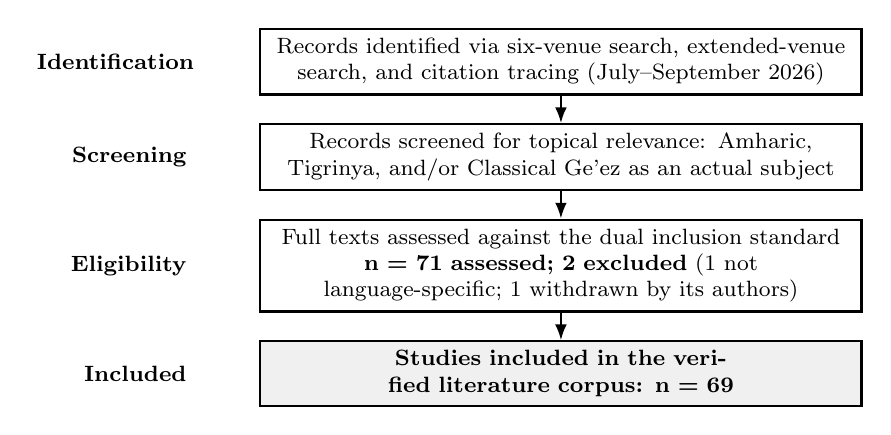
\begin{tikzpicture}[
  node distance=0.35cm and 0.8cm,
  box/.style={rectangle, draw, thick, text width=7.4cm, align=center, minimum height=0.8cm, font=\footnotesize},
  finalbox/.style={rectangle, draw, thick, fill=gray!12, text width=7.4cm, align=center, minimum height=0.8cm, font=\footnotesize},
  stagelabel/.style={font=\bfseries\footnotesize, text width=1.9cm, align=right},
  arr/.style={-{Latex[length=2mm]}, thick}
]
  \node[box] (identified) {Records identified via six-venue search, extended-venue search, and citation tracing (July--September 2026)};
  \node[stagelabel, left=of identified] {Identification};
  \node[box, below=of identified] (screened) {Records screened for topical relevance: Amharic, Tigrinya, and/or Classical Ge'ez as an actual subject};
  \node[stagelabel, left=of screened] {Screening};
  \node[box, below=of screened] (eligibility) {Full texts assessed against the dual inclusion standard\\ \textbf{n = 71 assessed; 2 excluded} (1 not language-specific; 1 withdrawn by its authors)};
  \node[stagelabel, left=of eligibility] {Eligibility};
  \node[finalbox, below=of eligibility] (included) {\textbf{Studies included in the verified literature corpus: n = 69}};
  \node[stagelabel, left=of included] {Included};
  \draw[arr] (identified) -- (screened);
  \draw[arr] (screened) -- (eligibility);
  \draw[arr] (eligibility) -- (included);
\end{tikzpicture}
\Description{Flow diagram of four stacked boxes connected by downward arrows, labelled Identification, Screening, Eligibility and Included. Identification: records found through the six-venue search, the extended-venue search and citation tracing, July to September 2026. Screening: records screened for Amharic, Tigrinya or Classical Ge'ez as an actual subject. Eligibility: 71 full texts assessed against the dual inclusion standard, 2 excluded. Included: 69 studies in the verified literature corpus.}
\caption{PRISMA 2020 flow diagram. Counts are reported only for the stages documented in the repository's version history; no preserved search log supports counts at the Identification or Screening stages, so none are asserted.}\label{fig:prisma-flow}
\end{figure}

\subsection{The Dual Inclusion Standard}\label{sec:dual-standard}

Screening literature by peer-review status while harvesting tools from GitHub, Zenodo, PyPI, and HuggingFace would be contradictory if left unstated: a tool's public existence and its peer-review status are independent properties. MoVoC~\cite{teklehaymanot_movoc_2025} and LGSE~\cite{teklehaymanot_lgse_2026}, for example, are peer-reviewed but had no confirmable release of their reported artefacts, whereas HornMorpho~\cite{gasser_hornmorpho_2011} is a maintained public repository whose paper predates the review window. We therefore use two standards that are never merged:
\begin{itemize}
  \item \textbf{Literature standard (two tracks).} Applies to the literature corpus (Sect.~\ref{sec:literature}). A paper is admitted through the peer-review track or the provenance track defined above; each paper's track is recorded in the corpus file. Related work may additionally cite background sources outside the corpus.
  \item \textbf{Tool-inventory standard (provenance-based).} Applies to the inventory (Sect.~\ref{sec:inventory}). Any code repository, dataset, or model with a stable, citable public identifier (a DOI, a GitHub repository, a HuggingFace card, or a Zenodo record) is eligible regardless of peer-review status.
\end{itemize}
The provenance track admits a \emph{paper} that describes an artefact; the tool-inventory standard admits an \emph{artefact} with a public identifier. ``Verified'' means that an entry's bibliographic details, or for a tool its repository link, were independently confirmed to exist and to match the source. It does not mean that data quality was assessed: this survey does not re-annotate or audit any dataset (Sect.~\ref{sec:limitations}).

\subsection{Tool Discovery and Verification}\label{sec:tool-discovery}

For every corpus paper that reports creating a tool, model, dataset, or resource, we searched GitHub, Zenodo, PyPI, and HuggingFace for that specific artefact. An artefact is counted only when a live link to the artefact the paper reports was confirmed; a link to a different or later artefact, even under the same author's account, does not qualify.\footnote{For example, the HuggingFace Space \texttt{Hailay/movoc-tok-playground} hosts a later tokenizer described by its model card as ``a continuation of MoVoC'', not the artefact the MoVoC paper reports, and is therefore not counted.} This yielded 26 corpus-traceable tools. The search is corpus-first: no repository search was run independently of the corpus, so the inventory is not an exhaustive census. Two well-known tools found outside the corpus are added under the provenance-based standard, each to fill a pillar with no corpus-traceable tool: HornMorpho (P2) and MasakhaNER~1.0~\cite{adelani_masakhaner_2021} (P4), giving 28. Every repository link is checked by a committed script that records a timestamped log. The inventory is frozen at its verification date (21 September 2026); later releases are recorded in a repository addenda file but not counted here.

%% ======================================================================
\section{Related Work}\label{sec:related}

Joshi et al.~\cite{joshi_state_2020} document the underrepresentation of most of the world's languages in NLP, and Blodgett et al.~\cite{blodgett_language_2021} connect such gaps to linguistic inequality. For Ge'ez-script languages, Gaim and Park~\cite{gaim_tigrinya_2025} survey Tigrinya NLP across 15 tasks, and Tonja et al.~\cite{tonja_natural_2023} survey four Ethiopian languages and consolidate their resources in a central repository. Neither reports a tool inventory scoped to Ge'ez-script languages and checked against live repository sources, which is the contribution of the present work. Methodologically, we follow the PRISMA 2020 reporting guideline~\cite{page_prisma_2021} as far as our preserved evidence allows, and extend it with a separately governed tool inventory.

%% ======================================================================
\section{The Reviewed Literature}\label{sec:literature}

Table~\ref{tab:literature} characterises the 69 papers, tallied directly from the corpus file. Amharic dominates (68\%), Tigrinya follows (38\%), and Classical Ge'ez is least represented (20\%). By pillar, P3 accounts for nearly half of the corpus (48\%) and infrastructure and resource papers for a further 38\%, while P1 (1\%) and P2 (4\%) are markedly underrepresented relative to their importance for Ge'ez-script morphology. Publication activity is concentrated in 2022--2026 (59\%).

\begin{table}[t]
\centering
\caption{The 69-paper literature corpus by language (overlapping counts), pillar, and period}\label{tab:literature}
\footnotesize
\begin{tabular}{@{}lrr@{\hspace{1.2em}}lrr@{\hspace{1.2em}}lrr@{}}
\toprule
\textbf{Language} & \textbf{n} & \textbf{\%} & \textbf{Pillar} & \textbf{n} & \textbf{\%} & \textbf{Period} & \textbf{n} & \textbf{\%}\\
\midrule
Amharic & 47 & 68 & P1 Tokenisation & 1 & 1 & 2016--2018 & 5 & 7\\
Tigrinya & 26 & 38 & P2 Morphology & 3 & 4 & 2019--2021 & 23 & 33\\
Classical Ge'ez & 14 & 20 & P3 Embeddings/eval. & 33 & 48 & 2022--2024 & 27 & 39\\
 & & & P4 Seq.\ labelling & 6 & 9 & 2025--2026 & 14 & 20\\
 & & & Other/infrastructure & 26 & 38 & & & \\
\bottomrule
\end{tabular}
\end{table}

Application papers are included only through their artefact or algorithmic contribution (Sect.~\ref{sec:literature-search}): for example, fake-news datasets~\cite{gereme_combating_2021}, speech and speech-emotion corpora~\cite{abera_designtigrinya_2018,retta_new_2023,assfaw_dialectbased_2022}, OCR datasets and pipelines~\cite{beyene_handwritten_2019,negashe_modified_2020}, and bias-evaluation studies, which fall under P3~\cite{zenebe_genderbias_2024,sewunetie_genderbias_2024}. Large multilingual works in which a Ge'ez-script language is one of many (e.g.\ AfroXLMR~\cite{alabi_adapting_2022}, MasakhaPOS~\cite{dione_masakhapos_2023}) are excluded under the language-focus criterion.

%% ======================================================================
\section{The Tool Inventory}\label{sec:inventory}

Table~\ref{tab:inventory} lists the 28 verified tools. Summed over the corpus, papers report 75 artefacts across 53 papers; 26 of these, from 17 papers, have a confirmed live release. The others are described in their papers but have no confirmable public link, or were excluded as general-purpose multilingual models without Ge'ez-script-specific adaptation. EthioLLM's benchmark is listed per dataset because language coverage differs between its constituents~\cite{tonja_ethiollm_2024}. Oromo, covered by several tools, is written in Latin script (Qubee)~\cite{tegegne_qubee_2016} and is outside scope even where a tool also covers in-scope languages.

\begin{table}[!t]
\centering
\caption{The 28 verified tools. Languages: Amh = Amharic, Tir = Tigrinya, Gez = Classical Ge'ez (out-of-scope languages also covered are omitted). The full table with exact repository identifiers and verification log is in the public repository.}\label{tab:inventory}
\scriptsize
\setlength{\tabcolsep}{3pt}
\begin{tabularx}{\textwidth}{@{}l>{\raggedright\arraybackslash}Xllll@{}}
\toprule
\textbf{Source} & \textbf{Name} & \textbf{Type} & \textbf{Lang.} & \textbf{Pillar} & \textbf{Host}\\
\midrule
\cite{mekonnen_optimized_2025} & amharic-ir-benchmarks & Library & Amh & P3 & GitHub\\
\cite{mekonnen_optimized_2025} & roberta-amharic-text-embedding (base, medium) & Model $\times$2 & Amh & P3 & HF\\
\cite{mekonnen_optimized_2025} & ColBERT-Mini (Amharic) & Model & Amh & P3 & HF\\
\cite{tonja_ethiollm_2024} & EthioPOS / EthioSenti / EthioHate & Dataset $\times$3 & Amh,Tir,Gez / Tir / Amh & P3 & HF\\
\cite{tonja_ethiollm_2024} & EthioLLM model family & Model & Amh,Tir,Gez & P3 & HF\\
\cite{yimam_exploring_2020} & Amharic sentiment dataset & Dataset & Amh & P3 & GitHub\\
\cite{yimam_introducing_2021} & amseg & Library & Amh & P1 & GitHub+PyPI\\
\cite{yohannes_named-entity_2022} & Tigrinya NER dataset & Dataset & Tir & P4 & GitHub\\
\cite{gaim_geezswitch_2022} & GeezSwitch / GeezSwitch-data & Library, Dataset & Amh,Tir,Gez & Other & GitHub\\
\cite{seyoum_universal_2018} & Amharic UD Treebank & Ling.\ resource & Amh & P4 & GitHub\\
\cite{abedissa_amqa_2023} & AmQA & Dataset & Amh & P3 & GitHub+HF\\
\cite{azime_proverbeval_2024} & EthioProverbEval / ProverbEval benchmark & Library, Dataset & Amh,Tir,Gez & P3 & GitHub, HF\\
\cite{gaim_multitask_2025} & TiALD / TiALD dataset & Library, Dataset & Tir & Other & GitHub, HF\\
\cite{gaim_tlmd_2021} & TLMD & Dataset & Tir & Other & Zenodo\\
\cite{gaim_monolingual_2021} & Tigrinya PLMs (TiBERT, TiELECTRA, TiRoBERTa) & Model & Tir & P3 & HF\\
\cite{azime_waliallm_2024} & Walia-LLM & Model & Amh & P3 & HF\\
\cite{yeshambel_2airtc_2020} & 2AIRTC & Dataset & Amh & Other & HF\\
\cite{belay_enhancing_2026} & EthioEmo-intensities & Dataset & Amh,Tir & P3 & GitHub+HF\\
\cite{retta_new_2023} & ASED & Dataset & Amh & Other & GitHub\\
\cite{mersha_morphologyrich_2020} & amharic\_word\_\allowbreak embeddings & Dataset+Model & Amh & P3 & GitHub\\
\midrule
\multicolumn{6}{@{}l}{\emph{Provenance-track additions (originating paper outside the corpus)}}\\
\cite{gasser_hornmorpho_2011} & HornMorpho & Library & Amh,Tir & P2 & GitHub\\
\cite{adelani_masakhaner_2021} & MasakhaNER 1.0 & Dataset & Amh & P4 & GitHub+HF\\
\bottomrule
\end{tabularx}
\end{table}

\begin{table}[t]
\centering
\caption{The 28 tools by pillar and by language (overlapping counts)}\label{tab:overview}
\footnotesize
\begin{tabular}{@{}lrr@{\hspace{2em}}lrr@{}}
\toprule
\textbf{Pillar} & \textbf{n} & \textbf{\%} & \textbf{Language} & \textbf{n} & \textbf{\%}\\
\midrule
P1 Tokenisation \& normalisation & 1 & 4 & Amharic & 22 & 79\\
P2 Morphological analysis \& synthesis & 1 & 4 & Tigrinya & 14 & 50\\
P3 Embeddings, LMs \& evaluation & 16 & 57 & Classical Ge'ez & 6 & 21\\
P4 Sequence labelling & 3 & 11 & & & \\
Other: infrastructure & 7 & 25 & & & \\
\midrule
Total & 28 & 100 & & & \\
\bottomrule
\end{tabular}
\end{table}

\subsubsection{Pillars.} P3 dominates (16 of 28; Table~\ref{tab:overview}), reflecting the trend towards pre-trained models and dense retrieval. P1 has a single verified tool, the Amharic-only amseg. No P2 tool from the corpus itself has a confirmed release: morphology-focused artefacts are described in the reviewed papers~\cite{gidey_morphological_2024,gebremeskel_tigrigna_2023,nigusie_suffixinflectional_2024}, but no public link could be confirmed, and the single P2 tool is the provenance-track addition HornMorpho. P4 has three tools; further sequence-labelling artefacts, such as TiNC24~\cite{berhane_towards_2025} and ANEC~\cite{jibril_anec_2022}, have no confirmable public release.

\subsubsection{Languages.} Amharic is supported by 22 tools (79\%), Tigrinya by 14 (50\%), and Classical Ge'ez by 6 (21\%). No tool is dedicated to Classical Ge'ez alone: all six Ge'ez-supporting tools also cover both Amharic and Tigrinya.

%% ======================================================================
\section{Research Asymmetry}\label{sec:asymmetry}

Amharic is the most represented language in both the literature (68\% of 69 papers) and the inventory (79\% of 28 tools); Tigrinya is second (38\%; 50\%); and Classical Ge'ez is least represented (20\%; 21\%). Eight tools cover more than one of the three languages: EthioPOS, the EthioLLM model family, GeezSwitch, GeezSwitch-data, EthioProverbEval, and the ProverbEval benchmark cover all three, and EthioEmo-intensities and HornMorpho cover Amharic and Tigrinya. Most are multilingual resources for Ethiopian languages in general, and only GeezSwitch and GeezSwitch-data are designed around the script itself. None is a script-level transfer framework, and they follow no shared annotation or evaluation conventions. LGSE~\cite{teklehaymanot_lgse_2026} and MoVoC~\cite{teklehaymanot_movoc_2025} propose cross-lingual components for these languages, but neither had a confirmable release of its reported artefact at the verification date.\footnote{A release matching MoVoC's corrected version (ACL Anthology revision~2, 21 October 2026) has since appeared and is recorded in the repository's inventory addenda.}

%% ======================================================================
\section{Limitations}\label{sec:limitations}

\subsubsection{Search.} No query-level log was preserved, so counts before full-text assessment are not reported (Fig.~\ref{fig:prisma-flow}). The search favours published and NLP-venue work, and English-language publications. Some in-scope work was not captured, including Tigrinya part-of-speech tagging on the Nagaoka Tigrinya Corpus~\cite{tedla_tigrinya_2016}, LSTM-based Tigrinya morphological segmentation~\cite{tedla_morphological_2018}, and deep-learning part-of-speech tagging for Tigrinya and Tigre~\cite{kapociute_northern_2020}. These fall in P2 and P4; adding them would leave P1 and P2 the least-represented pillars.

\subsubsection{Coding.} Formal double-coding with an inter-rater agreement statistic was not performed (Sect.~\ref{sec:literature-search}).

\subsubsection{Inventory.} The inventory is corpus-first and frozen at its verification date; an artefact whose public release could not be confirmed is not counted, even when its paper asserts one.

\subsubsection{Data Quality.} Verification establishes existence and provenance only. Annotation quality, agreement, and label correctness of the catalogued datasets are not assessed.

%% ======================================================================
\section{Research Priorities}\label{sec:agenda}

The first five priorities follow from the gaps in Sects.~\ref{sec:literature}--\ref{sec:asymmetry}; the last two address a limitation of this survey and a scope boundary of its search.


\subsubsection{Priority 1: Shared Tokenisation.} P1 holds 1 of 28 tools and 1 of 69 papers, and that tool is Amharic-only. A tokeniser evaluated jointly on all three languages, with a documented public release, is the clearest gap.

\subsubsection{Priority 2: Morphology with a Verifiable Release.} Three corpus papers describe P2 tools~\cite{gidey_morphological_2024,gebremeskel_tigrigna_2023,nigusie_suffixinflectional_2024} without a confirmable release. Publishing such a tool with a stable identifier, or extending HornMorpho rather than duplicating it, would close this gap.

\subsubsection{Priority 3: Balance Against P3.} P3 holds 57\% of tools and 48\% of papers; new work on P1, P2, or P4 adds more than further P3 work.

\subsubsection{Priority 4: Releases for Sequence Labelling.} P4 artefacts already described in the literature (e.g.\ TiNC24, ANEC) could be released under stable identifiers without new research.

\subsubsection{Priority 5: Cross-Language Coordination.} Shared annotation and evaluation conventions would let tools reuse resources across the three languages instead of duplicating single-language work.

\subsubsection{Priority 6: Independent Data-Quality Assessment.} Catalogued datasets should be adopted only after their annotation methodology and quality metrics are reviewed; a systematic quality audit of the inventory is a natural follow-up.

\subsubsection{Priority 7: Reuse of Classical Semitic Studies and Digital Humanities.} Our search is scoped to NLP venues. Long-running philological and digital-humanities projects, often funded by research councils, produced manuscript digitisations, digital editions, Unicode transcriptions, TEI annotation workflows, tagging manuals, and parsers, but these have rarely reached working tools for the communities that use the script. Much of this material was processed in Latin transliteration. For example, the Ge'ez Morphological Parser~\cite{liuzzo_geez_2019}, developed in the ERC-funded TraCES project, is being redeveloped under the SNSF-funded MiTAnIm project. Adapting such resources, and converting transliterated material back into the Ge'ez script, would advance all four pillars without building from scratch~\cite{digitalorientalist2026}.

%% ======================================================================
\section{Conclusion}\label{sec:conclusion}

This survey documents 28 foundational tools, models, datasets, and linguistic resources confirmed publicly available for Amharic, Tigrinya, and Classical Ge'ez, alongside a PRISMA-guided review of 69 verified papers. Amharic dominates both the literature and the inventory, and Classical Ge'ez is least served. Tokenisation and morphology are the thinnest pillars: P1 has a single, Amharic-only tool, and no corpus paper's own morphological tool has a confirmed release. Eight tools span more than one language, but none is a shared framework. The seven priorities above, from a joint tokeniser to the reuse of digital-humanities resources, target these gaps. All data, the full inventory, and the verification code are public.

\begin{credits}
\subsubsection{\ackname} This review was conducted as part of research on low-resource language technology at the L3S Research Center, Leibniz University Hannover. We thank the Ge'ez-script NLP community, particularly contributors to the LGSE Project and the Masakhane initiative.

\subsubsection{\discintname}
The authors have no competing interests to declare that are relevant to the content of this article.
\end{credits}

\bibliographystyle{splncs04}
\bibliography{../references}

\end{document}
